% Options for packages loaded elsewhere
\PassOptionsToPackage{unicode}{hyperref}
\PassOptionsToPackage{hyphens}{url}
%
\documentclass[
  ignorenonframetext,
  aspectratio=169]{beamer}
\usepackage{pgfpages}
\setbeamertemplate{caption}[numbered]
\setbeamertemplate{caption label separator}{: }
\setbeamercolor{caption name}{fg=normal text.fg}
\beamertemplatenavigationsymbolsempty
% Prevent slide breaks in the middle of a paragraph
\widowpenalties 1 10000
\raggedbottom
\setbeamertemplate{part page}{
  \centering
  \begin{beamercolorbox}[sep=16pt,center]{part title}
    \usebeamerfont{part title}\insertpart\par
  \end{beamercolorbox}
}
\setbeamertemplate{section page}{
  \centering
  \begin{beamercolorbox}[sep=12pt,center]{part title}
    \usebeamerfont{section title}\insertsection\par
  \end{beamercolorbox}
}
\setbeamertemplate{subsection page}{
  \centering
  \begin{beamercolorbox}[sep=8pt,center]{part title}
    \usebeamerfont{subsection title}\insertsubsection\par
  \end{beamercolorbox}
}
\AtBeginPart{
  \frame{\partpage}
}
\AtBeginSection{
  \ifbibliography
  \else
    \frame{\sectionpage}
  \fi
}
\AtBeginSubsection{
  \frame{\subsectionpage}
}
\usepackage{amsmath,amssymb}
\usepackage{iftex}
\ifPDFTeX
  \usepackage[T1]{fontenc}
  \usepackage[utf8]{inputenc}
  \usepackage{textcomp} % provide euro and other symbols
\else % if luatex or xetex
  \usepackage{unicode-math} % this also loads fontspec
  \defaultfontfeatures{Scale=MatchLowercase}
  \defaultfontfeatures[\rmfamily]{Ligatures=TeX,Scale=1}
\fi
\usepackage{lmodern}
\ifPDFTeX\else
  % xetex/luatex font selection
\fi
% Use upquote if available, for straight quotes in verbatim environments
\IfFileExists{upquote.sty}{\usepackage{upquote}}{}
\IfFileExists{microtype.sty}{% use microtype if available
  \usepackage[]{microtype}
  \UseMicrotypeSet[protrusion]{basicmath} % disable protrusion for tt fonts
}{}
\makeatletter
\@ifundefined{KOMAClassName}{% if non-KOMA class
  \IfFileExists{parskip.sty}{%
    \usepackage{parskip}
  }{% else
    \setlength{\parindent}{0pt}
    \setlength{\parskip}{6pt plus 2pt minus 1pt}}
}{% if KOMA class
  \KOMAoptions{parskip=half}}
\makeatother
\usepackage{xcolor}
\newif\ifbibliography
\usepackage{listings}
\newcommand{\passthrough}[1]{#1}
\lstset{defaultdialect=[5.3]Lua}
\lstset{defaultdialect=[x86masm]Assembler}
\setlength{\emergencystretch}{3em} % prevent overfull lines
\providecommand{\tightlist}{%
  \setlength{\itemsep}{0pt}\setlength{\parskip}{0pt}}
\setcounter{secnumdepth}{-\maxdimen} % remove section numbering
\setbeamersize{text margin left=0.35cm}
\setbeamersize{text margin right=0.35cm}

\definecolor{peach}{HTML}{EDD1B0}
\setbeamercolor{background canvas}{bg=peach}


\let\oldverbatim\verbatim
\let\oldendverbatim\endverbatim
\renewenvironment{verbatim}{\scriptsize\oldverbatim}{\oldendverbatim}

% \renewenvironment{Shaded}{\begin{snugshade}\footnotesize}{\end{snugshade}}

\setbeamertemplate{itemize item}{>}
\setbeamertemplate{itemize subitem}{--}

\setbeamerfont{itemize/enumerate body}{size=\large}
\setbeamerfont{itemize/enumerate subbody}{size=\large}
\setbeamerfont{itemize/enumerate subsubbody}{size=\small}

% \setbeamerfont{normal text}{size=\large}
\AtBeginDocument{\large}


\usepackage{listings}
\lstset{basicstyle=\small}

\setbeamertemplate{footline}[page number]
\ifLuaTeX
  \usepackage{selnolig}  % disable illegal ligatures
\fi
\usepackage{bookmark}
\IfFileExists{xurl.sty}{\usepackage{xurl}}{} % add URL line breaks if available
\urlstyle{same}
\hypersetup{
  pdftitle={Elixir\textquotesingle s Set-Theoretic Type System},
  pdfauthor={Robert Ellen},
  hidelinks,
  pdfcreator={LaTeX via pandoc}}

\title{Elixir\textquotesingle s Set-Theoretic Type System}
\author{Robert Ellen}
\date{2024/11/12}

\begin{document}
\frame{\titlepage}

\section{Summary}\label{summary}

\section{Elixir}\label{elixir-1}

\begin{frame}{Elixir}


\end{frame}

\section{The Erlang Ecosystem}\label{the-erlang-ecosystem}

\begin{frame}{What is the Erlang Ecosystem?}
\phantomsection\label{what-is-the-erlang-ecosystem}
A group of languages, libraries, frameworks, and applications that are
implemented on top of the Erlang virtual machine, the BEAM.

Languages include:

\begin{figure}
\centering
\begin{minipage}{.24\textwidth}
  \centering
  
\includegraphics[width=.8\linewidth]{./img/erlang_logo.png}
\end{minipage}
\begin{minipage}{.24\textwidth}
  \centering
  
\includegraphics[width=.8\linewidth]{./img/elixir-vertical.png}
\end{minipage}
\begin{minipage}{.24\textwidth}
  \centering
  
\includegraphics[width=.8\linewidth]{./img/lucy.png}
\end{minipage}
\begin{minipage}{.24\textwidth}
  \centering
  
\includegraphics[width=.8\linewidth]{./img/lfe.png}
\end{minipage}
\end{figure}

\ldots plus dozens more
\end{frame}

\begin{frame}{What is the Erlang Ecosystem?}
\phantomsection\label{what-is-the-erlang-ecosystem-1}
Libraries and frameworks include:

\begin{figure}
\centering
\begin{minipage}{.24\textwidth}
  \centering
 \LARGE{OTP}
\end{minipage}
\begin{minipage}{.24\textwidth}
  \centering
  
\includegraphics[width=.8\linewidth]{./img/rabbitmq_logo.png}
\end{minipage}
\begin{minipage}{.24\textwidth}
  \centering
  
\includegraphics[width=.8\linewidth]{./img/phoenix_logo.png}
\end{minipage}
\begin{minipage}{.24\textwidth}
  \centering
  
\includegraphics[width=.8\linewidth]{./img/ecto_logo.png}
\end{minipage}
\begin{minipage}{.24\textwidth}
\centering
  
\includegraphics[width=.8\linewidth]{./img/absinthe_logo.png}
\end{minipage}
\begin{minipage}{.24\textwidth}
\centering
  
\includegraphics[width=.8\linewidth]{./img/oban-logo.png}
\end{minipage}
\begin{minipage}{.24\textwidth}
  \centering
  
\includegraphics[width=.7\linewidth]{./img/nx_logo.png}
\end{minipage}
\begin{minipage}{.24\textwidth}
  \centering
  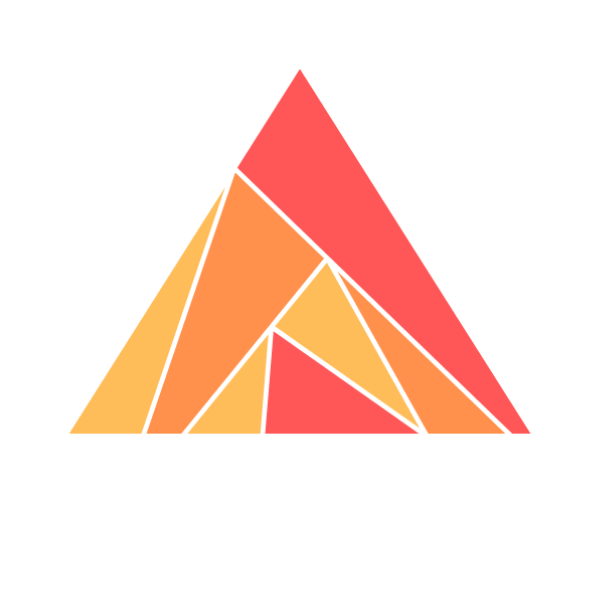
\includegraphics[width=.8\linewidth]{./img/ash-logo.png}
\end{minipage}
\end{figure}
\end{frame}

\begin{frame}{What is the Erlang Ecosystem?}
\phantomsection\label{what-is-the-erlang-ecosystem-2}
Built around a shared value in:

\begin{itemize}
\tightlist
\item
  massive concurrency
\item
  fault-tolerance
\item
  simplicity
\item
  acknowledging the errors will occur so let\textquotesingle s deal with
  them

  \begin{itemize}
  \tightlist
  \item
    ``Let it crash"--have a plan to restart sub-systems when they crash
  \end{itemize}
\end{itemize}
\end{frame}

\section{A brief history of Erlang}\label{a-brief-history-of-erlang}

\begin{frame}{A brief history of Erlang}
\phantomsection\label{a-brief-history-of-erlang-1}
\centering
covered in my 2013 talk, but tonight...
\end{frame}

\begin{frame}{A brief history of Erlang}
\phantomsection\label{a-brief-history-of-erlang-2}
\begin{center}

\includegraphics[width=.5\textwidth]{./img/short_short.jpg}
\end{center}
\end{frame}

\begin{frame}{A brief history of Erlang}
\phantomsection\label{a-brief-history-of-erlang-3}
\begin{itemize}
\tightlist
\item
  developed in the mid 1980s at Ericsson
\item
  to run on next generation telephone switches

  \begin{itemize}
  \tightlist
  \item
    concurrent, fault-tolerant, distributed, soft real-time
  \item
    strong, dynamically typed, impure, functional, simple
  \item
    reports of 1200k LOC and ``nine nines" of uptime on the AXD301
    switch
  \item
    reports of market penetration of \textgreater{} 50\% in mobile
    telephony switches
  \end{itemize}
\item
  solved web-scale in the \textquotesingle80s
\end{itemize}

\begin{figure}
\centering
\vspace{20pt}
\begin{minipage}{.24\textwidth}
  \centering
  
\includegraphics[width=.9\linewidth]{./img/joe.jpg}
\end{minipage}
\begin{minipage}{.24\textwidth}
  \centering
  
\includegraphics[width=.9\linewidth]{./img/mike.jpeg}
\end{minipage}
\begin{minipage}{.24\textwidth}
  \centering
  
\includegraphics[width=.9\linewidth]{./img/robert.jpeg}
\end{minipage}
\begin{minipage}{.24\textwidth}
  \centering
  
\includegraphics[width=.9\linewidth]{./img/bjarne.jpg}
\end{minipage}
\end{figure}
\end{frame}

\section{The BEAM and OTP}\label{the-beam-and-otp}

\begin{frame}{The BEAM}
\phantomsection\label{the-beam}
\begin{itemize}
\tightlist
\item
  Erlang\textquotesingle s virtual machine / runtime system
\item
  lightweight processes, SMP, low-latency IO, soft realtime, minimal
  locks
\item
  multi-generational, per-process garbage collector
\item
  asynchronous, location-transparent, message passing IPC
\item
  hot-code-loading
\item
  powerful REPL and introspection tools
\item
  new JIT compiler (BEAM bytecode to machine code)
\end{itemize}
\end{frame}

\begin{frame}[fragile]{The OTP libraries}
\phantomsection\label{the-otp-libraries}
\begin{itemize}
\tightlist
\item
  Erlang\textquotesingle s ``standard library"
\item
  dozens of modules providing various typical stdlib stuff
\item
  core of which are for supervision trees

  \begin{itemize}
  \tightlist
  \item
    \passthrough{\lstinline!gen\_server!} - actors / workers
  \item
    supervisors - handling starting/stopping/restarting
    \passthrough{\lstinline!gen\_servers!}
  \end{itemize}
\end{itemize}
\end{frame}

\begin{frame}{supervision trees}
\phantomsection\label{supervision-trees}
\begin{center}
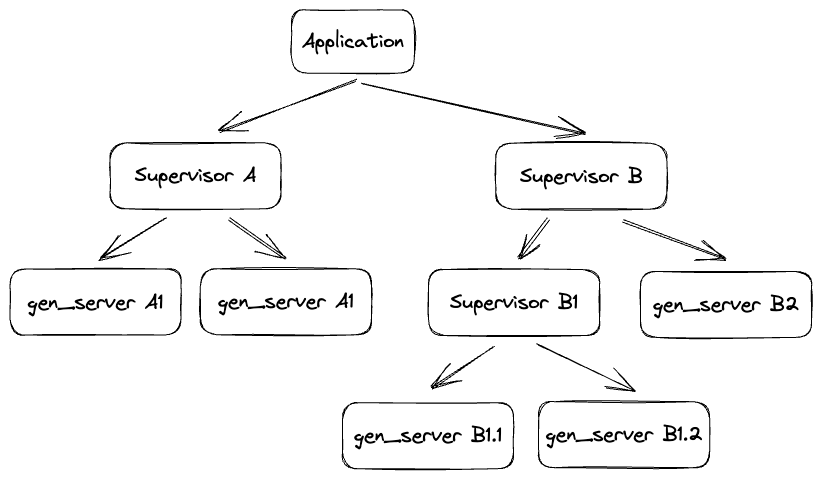
\includegraphics[width=0.8\textwidth]{./img/tree.png}
\end{center}
\end{frame}

\begin{frame}{Elixir}
\phantomsection\label{elixir}
There will be some comparing and contrasting of Gleam with
Elixir\ldots{}

\begin{center}

\includegraphics[width=.5\textwidth]{./img/elixir_logo.png}
\end{center}
\end{frame}

\begin{frame}{Brief history of Elixir}
\phantomsection\label{brief-history-of-elixir}
\begin{itemize}
\tightlist
\item
  created by José Valim starting in 2012
\item
  inspired by Erlang, Ruby, and, to a lesser extent, Lisp
\item
  like Erlang, the language is quite stable, imminent release of v1.18
\item
  has gone from web applications to embedded systems and numerical
  analysis and ML/AI
\end{itemize}

\begin{center}

\includegraphics[width=.5\textwidth]{./img/elixir_logo.png}
\end{center}
\end{frame}

\begin{frame}[fragile]{Features of Elixir}
\phantomsection\label{features-of-elixir}
\begin{itemize}
\tightlist
\item
  Ruby-like syntax while retaining most of Erlang\textquotesingle s
  semantics

  \begin{itemize}
  \tightlist
  \item
    \ldots, immutable data, HoF, side-effects anywhere,
    dynamically-typed, \ldots{}
  \end{itemize}
\item
  interoperate with Erlang
\item
  hygienic macros
\item
  ad-hoc polymorhism with protocols
\item
  highly ergonomic build tool: \passthrough{\lstinline!mix!}
\item
  modern package manager: \passthrough{\lstinline!hex!}
\item
  excellent unit test tool: exunit
\item
  opinionated formatter
\item
  did I mention dynamically-typed?
\end{itemize}
\end{frame}

\section{Typing BEAM languages}\label{typing-beam-languages}

\begin{frame}{Marlow \& Wadler - 1997}
\phantomsection\label{marlow-wadler---1997}
\centering
``We can stop waiting for functional languages to be used in practice--that day is here!"

\begin{itemize}
\tightlist
\item
  threw away Hindley-Milner: \(U = V\) -- this would not work with
  existing Erlang codebases
\item
  opted for strictly more general ``semantic sub-typing" instead:
  \(U \subseteq V\)
\item
  this approach developed by Aiken \& Wimmers 1993
\end{itemize}
\end{frame}

\begin{frame}{eqWAlizer}
\phantomsection\label{eqwalizer}
\begin{itemize}
\tightlist
\item
  Developed by Meta for WhatsApp
\item
  set-theoretic gradual typing
\item
  \url{https://github.com/WhatsApp/eqwalizer}
\end{itemize}
\end{frame}

\begin{frame}{Static analysis tools}
\phantomsection\label{static-analysis-tools}
\begin{itemize}
\tightlist
\item
  rely on the Erlang Typespec notation - not checked by compiler
\item
  dialyzer

  \begin{itemize}
  \tightlist
  \item
    success-typing based on whole-program analysis
  \item
    will only fail if it can prove there\textquotesingle s a problem (no
    false positives)
  \item
    Linhahl \& Sagonas, 2006
  \end{itemize}
\item
  gradualizer - gradual set-theoretic-inspired typing
\end{itemize}
\end{frame}

\begin{frame}{Typed BEAM languages with alternate semantics}
\phantomsection\label{typed-beam-languages-with-alternate-semantics}
\begin{itemize}
\tightlist
\item
  Hamler - PureScript for the BEAM
\item
  Caramel - ML for the BEAM
\item
  Gleam - Rust/Ocaml/Elm inspired - HM type system

  \begin{itemize}
  \tightlist
  \item
    see my May 2024 talk
  \end{itemize}
\item
  \ldots{}
\end{itemize}
\end{frame}

\section{Elixir\textquotesingle s set-theoretic type
system}\label{elixirs-set-theoretic-type-system-7}

\begin{frame}{Elixir\textquotesingle s set-theoretic type system}
\phantomsection\label{elixirs-set-theoretic-type-system-8}
A research and development project to gradually introduce a static type
system to Elixir.

\small Giuseppe Castagna, Guillaume Duboc, and José Valim. The Design
Principles of the Elixir Type System The Art, Science, and Engineering
of Programming, 2024, Vol. 8, Issue 2, Article 4
\url{https://doi.org/10.22152/programming-journal.org/2024/8/4}
\end{frame}

\begin{frame}{Requirements}
\phantomsection\label{requirements}
\begin{itemize}
\tightlist
\item
  no modification to the syntax of Elixir expressions
\item
  gradual typing
\item
  extract maximum type information from patterns and guards
\item
  mode to emit warnings when explicitly using gradual typing
\item
  type annotations across language before advanced features
\item
  initially - typing does not modify the compilation of Elixir code
\end{itemize}
\end{frame}

\begin{frame}{Features of the type system}
\phantomsection\label{features-of-the-type-system}
\begin{itemize}
\tightlist
\item
  semantic subtyping hence set-theoretic
\item
  parametric polymorphism with local type inference

  \begin{itemize}
  \tightlist
  \item
    type variables
  \item
    requires some type annotations--but not everywhere
  \end{itemize}
\item
  use patterns and guards
\item
  typing maps in all use-cases
\item
  gradual typing
\item
  strong arrows
\item
  typing ad-hoc polymorphism
\end{itemize}
\end{frame}

\begin{frame}{Semantic subtyping}
\phantomsection\label{semantic-subtyping}
\begin{itemize}
\tightlist
\item
  establish subtyping relationships between types based on the semantic
  meaning of values of the types
\item
  semantic meaning derived from treating types as sets, values as set
  members
\item
  set operations on types: union, intersection, and negation
\item
  in comparison to Hindley-Milner, relax \(U = V\) to \(U \subseteq V\)
\item
  strictly more general--an extension to HM
\item
  Frish et. al. referencing Aiken \& Wimmers (also ref. by Marlow \&
  Wadler)
\item
  good idea because dynamically-typed languages variables can hold
  different types at run-time: hence union-ing
\end{itemize}
\end{frame}

\begin{frame}{Subtyping in type checking}
\phantomsection\label{subtyping-in-type-checking}
\begin{itemize}
\tightlist
\item
  subtyping is a means to typechecking programs due to ``subsumption"
\end{itemize}

\huge

\begin{center}
 $\frac{e : T_1 \quad T_1 <: T_2}{e : T_2}$
 \end{center}

\begin{itemize}
\tightlist
\item
  given some expression \(e\) and types \(T_1\) and \(T_2\), if the type
  of \(e\) is \(T_1\) and \(T_1\) is a subtype of \(T_2\) then \(e\) can
  be considered to also be of type \(T_2\)
\end{itemize}
\end{frame}

\begin{frame}{Set-theoretic type annotations}
\phantomsection\label{set-theoretic-type-annotations}
examples here
\end{frame}

\begin{frame}[fragile]{Polymorphic with local type inference}
\phantomsection\label{polymorphic-with-local-type-inference}
\begin{itemize}
\tightlist
\item
  type variables: \passthrough{\lstinline!a, b!} - no parentheses
\item
  local type inference

  \begin{itemize}
  \tightlist
  \item
    functions must have type annotations
  \item
    types are inferred for arguments and return types
  \end{itemize}
\end{itemize}
\end{frame}

\begin{frame}[fragile]{Polymorphic with local type inference}
\phantomsection\label{polymorphic-with-local-type-inference-1}
\begin{lstlisting}
$ (list(a), a -> b) -> list(b)
def map([], _), do: []
def map([x | xs], f), do:  [f.(x) | map(xs, f)]

x = map([1, 2, 3], &double/1)
# type system infers type of double and x
\end{lstlisting}
\end{frame}

\begin{frame}[fragile]{Guards and pattern-matching}
\phantomsection\label{guards-and-pattern-matching}
\begin{itemize}
\tightlist
\item
  Elixir has rich run-time testing of types
\item
  the type system can type captured variables and variables in guards
\end{itemize}

\begin{lstlisting}
def elem_at([x | rest] = xs, pos) when is_integer(pos) do...
\end{lstlisting}
\end{frame}

\begin{frame}[fragile]{Guards and pattern-matching}
\phantomsection\label{guards-and-pattern-matching-1}
\begin{itemize}
\tightlist
\item
  ``type narrowing" can check exhaustiveness of case expressions
\item
  type system is conservative: case branches must handle
  \passthrough{\lstinline!xs!} being any map or list
\end{itemize}

\begin{lstlisting}
def elem_at(xs, pos) when is_map(xs) or is_list(x) do
  case xs do
    %{} -> # get for map
    [] -> # get for list
    _ -> # redundant
  end
end
\end{lstlisting}
\end{frame}

\begin{frame}[fragile]{Maps as ``records" and ``dictionaries"}
\phantomsection\label{maps-as-records-and-dictionaries}
\begin{itemize}
\tightlist
\item
  maps can represent records, dictionaries, and structs
\end{itemize}

\begin{lstlisting}
ashley = %{name: "Ashley", age: 42}
# ashley :: %{:name => binary(), :age => integer()}

words = "The Elixir Type System ..."
word_count = wc(words) # :: %{optional(binary()) => integer()}
word_count["Elixir"] # 42

defstruct [:id , name: "", age: 0]
# %{
#   :__struct__ => :"User",
#   :id => term(),
#   :name => binary(),
#   :age => integer()
# }
\end{lstlisting}
\end{frame}

\begin{frame}[fragile]{Maps as ``records" and ``dictionaries"}
\phantomsection\label{maps-as-records-and-dictionaries-1}
\begin{itemize}
\tightlist
\item
  the type system treats maps as open or closed

  \begin{itemize}
  \tightlist
  \item
    open means there are potentially unknown keys
  \end{itemize}
\item
  strict or dynamic access changes type inference
\end{itemize}

\begin{lstlisting}
user.first_name # user :: %{:first_name => term(), ...}

middle = person["middle_name"]
# person :: %{optional("middle_name") => term(), ...} => %{...}
# middle :: binary() or nil

ashley = %{name: "Ashley", age: 42}
# ashley :: %{:name => binary(), :age => integer()}
\end{lstlisting}
\end{frame}

\begin{frame}[fragile]{Maps as ``records" and ``dictionaries"}
\phantomsection\label{maps-as-records-and-dictionaries-2}
\begin{itemize}
\tightlist
\item
  subtyping maps feels like structural subtyping\ldots{}
\end{itemize}

\begin{lstlisting}
ashley = %{name: "Ashley", age: 42}
# ashley :: %{:name => binary(), :age => integer()}

ashley_at_school = %{name: "Ashley", age: 42, gpa: 6.75}
# ashley_at_school :: %{:name => binary(),
#                       :age => integer(),
#                       :gpa => float()}

def enroll(%{name: _, age: _} = person) do ...
\end{lstlisting}

\begin{itemize}
\tightlist
\item
  the type system innovates semantic subtyping to handle maps

  \begin{itemize}
  \tightlist
  \item
    Castagna 2023
  \end{itemize}
\end{itemize}
\end{frame}

\begin{frame}[fragile]{Gradual typing with
\passthrough{\lstinline!dynamic()!}}
\phantomsection\label{gradual-typing-with-dynamic}
\begin{itemize}
\tightlist
\item
  as per requirements, avoid boiling the ocean in existing codebases
\item
  gradual typing: see TypeScript, gradualizer
\item
  a type that ``materialises" into any other type
\item
  a type that can be the subtype and supertype of any other type

  \begin{itemize}
  \tightlist
  \item
    \passthrough{\lstinline!term()!} can only be the later, so need a
    new type
  \end{itemize}
\item
  \passthrough{\lstinline!dynamic()!}
\end{itemize}
\end{frame}

\begin{frame}{Gradual typing with \passthrough{\lstinline!dynamic()!}}
\phantomsection\label{gradual-typing-with-dynamic-1}
\begin{itemize}
\tightlist
\item
  ``sound gradual typing" - Siek \& Taha 2006
\item
  in the presence of dynamic typing, partial static typing still works
\item
  a static type annotation/inference guarantees an expression either:

  \begin{itemize}
  \tightlist
  \item
    never returns
  \item
    returns a value of the static type
  \item
    emits a runtime exception
  \end{itemize}
\item
  necessitates the addition of runtime checks to the compiled program
\item
  Elixir innovation: as per requirements, no change to the compiled
  program
\end{itemize}
\end{frame}

\begin{frame}[fragile]{Halting \passthrough{\lstinline!dynamic()!}
propagation}
\phantomsection\label{halting-dynamic-propagation}
\begin{itemize}
\tightlist
\item
  VM and programmer type checks halt the propagation of
  \passthrough{\lstinline!dynamic()!}
\item
  functions with these checks are referred to as ``strong arrows"
\end{itemize}

\begin{lstlisting}
$ integer() -> integer()
def id_strong(x) when is_integer(x), do: x

$ integer() -> integer()
def id_weak(x), do: x

# due to "weak" vs "strong" arrows, the following
# is an acceptable type annotation for `ids(x)`
$ dynamic() -> {dynamic(), integer()}
def ids(x), do: {id_weak(x), id_strong(x)}
\end{lstlisting}
\end{frame}

\begin{frame}[fragile]{``Solving" the expression problem with protocols}
\phantomsection\label{solving-the-expression-problem-with-protocols}
\begin{itemize}
\tightlist
\item
  ``ad-hoc" polymorphism akin to typeclasses
\item
  the type system will union all implementations of
  \passthrough{\lstinline!String.Chars!} to define a type
  \passthrough{\lstinline!String.Chars.t()!}
\end{itemize}

\begin{lstlisting}
defmodule MyNewType do
  defstruct [:data]
end

defimpl String.Chars, for: MyNewType do
  def to_string(value) do ... end
end
\end{lstlisting}
\end{frame}

\begin{frame}[fragile]{``Solving" the expression problem with protocols}
\phantomsection\label{solving-the-expression-problem-with-protocols-1}
\begin{itemize}
\tightlist
\item
  combines with parametric polymorphism
\item
  please say it is so!
\end{itemize}

\begin{lstlisting}
# functory.ex
$ Functory.t(a), (a -> b) -> Functory.t(b)
    when a: term(),  b: term()
def map(xs, f)
...
# my_struct.ex
defimpl Functory, for: MyStruct do
  def map(xs, f) do ... end
end
\end{lstlisting}
\end{frame}

\begin{frame}{Gradually introducing the system}
\phantomsection\label{gradually-introducing-the-system}
\begin{itemize}
\tightlist
\item
  don\textquotesingle t discount the chance of a deal-breaker in prod
  code taking them back to the drawing board
\item
  phased approach to introducing the experimental system into production
  Elixir compiler

  \begin{itemize}
  \tightlist
  \item
    local inference of some Elixir types: v1.17
  \item
    type all Elixir data types and add typing of (and use information
    inferred from) pattern matching and guards: v1.18
  \item
    type annotations for functions: v1.?
  \end{itemize}
\end{itemize}
\end{frame}

\begin{frame}{References}
\phantomsection\label{references}
Aiken, A. and Wimmers, E. L. 93. Type inclusion constraints and type
inference. In Proceed- ings of the Seventh ACM Conference on Functional
Programming and Computer Architecture. Copenhagen, Denmark, 31--41

Giuseppe Castagna. Typing records, maps, and structs. Proc. ACM Program.
Lang., 7(ICFP), September 2023. \url{doi:10.1145/3607838}.

Giuseppe Castagna, Guillaume Duboc, and José Valim. The Design
Principles of the Elixir Type System The Art, Science, and Engineering
of Programming, 2024, Vol. 8, Issue 2, Article 4
\url{https://doi.org/10.22152/programming-journal.org/2024/8/4}

Alain Frisch, Giuseppe Castagna, and Véronique Benzaken. Semantic
subtyping: dealing set-theoretically with function, union, intersection,
and negation types. Journal of the ACM, 55(4):1--64, 2008.
\url{doi:10.1145/1391289.1391293}
\end{frame}

\begin{frame}{References}
\phantomsection\label{references-1}
Tobias Lindahl and Konstantinos Sagonas. Practical type inference based
on success typings. In ACM-SIGPLAN International Conference on
Principles and Practice of Declarative Programming, 2006.
\url{doi:10.1145/1140335.1140356}.

Simon Marlow and Philip Wadler. A practical subtyping system for erlang.
In Proceedings of the Second ACM SIGPLAN International Conference on
Functional Programming, ICFP '97, page 136--149, New York, NY, USA,
1997. Association for Computing Machinery.
\url{doi:10.1145/258948.258962}.

Jeremy G. Siek and Walid Taha. Gradual typing for functional languages.
In Scheme and Functional Programming Workshop, University of Chicago
Technical Report TR-2006-06, pages 81--92, 2006.
\end{frame}

\begin{frame}{Thank you}
\phantomsection\label{thank-you}
I\textquotesingle ll post slides soon.
\end{frame}

\end{document}
